\section{Procesadores Superescalares}\label{sec:superscalar}

Una implementación superescalar de la arquitectura de un procesador es aquella en la que las instrucciones comunes pueden iniciar su ejecución simultáneamente y ejecutarse de manera independiente. Estas implementaciones plantean complejos problemas de diseño relacionados con el cauce de instrucciones.

Lo esencial del enfoque superescalar es su habilidad para ejecutar instrucciones en diferentes cauces de manera independiente y concurrente. El concepto puede llevarse más lejos permitiendo que las instrucciones se ejecuten en un orden diferente al del programa.

\subsection{Superescalar frente a supersegmentado}

La supersegmentación aprovecha el hecho de que muchas etapas del cauce realizan tareas que requieren menos de medio ciclo de reloj. De este modo, doblando la velocidad de reloj interna se permite la realización de dos tareas en un ciclo de reloj externo.

Las etapas macro se dividen en el cauce segmentado en sub-etapas más pequeñas y se transmiten los datos a la mayor velocidad del ciclo de reloj.

El enfoque supersegmentado aumenta el grado de paralelismo e incrementa la aceleración percibida.

El enfoque superescalar permite llevar a cabo más de una instrucción de manera simultánea. Conlleva la duplicación de algunas o todas las partes de la CPU/ALU.\@ Debe ser capaz de captar múltiples instrucciones al mismo tiempo. Ejecutar sumas y multiplicaciones simultáneamente. Ejecutar carga/almacenamiento, mientras se lleva a cabo una operación en ALU.\@ El grado de paralelismo y, por tanto, la aceleración de la máquina aumenta, ya que se ejecutan más instrucciones en paralelo.

\begin{figure}[H]
  \centering
  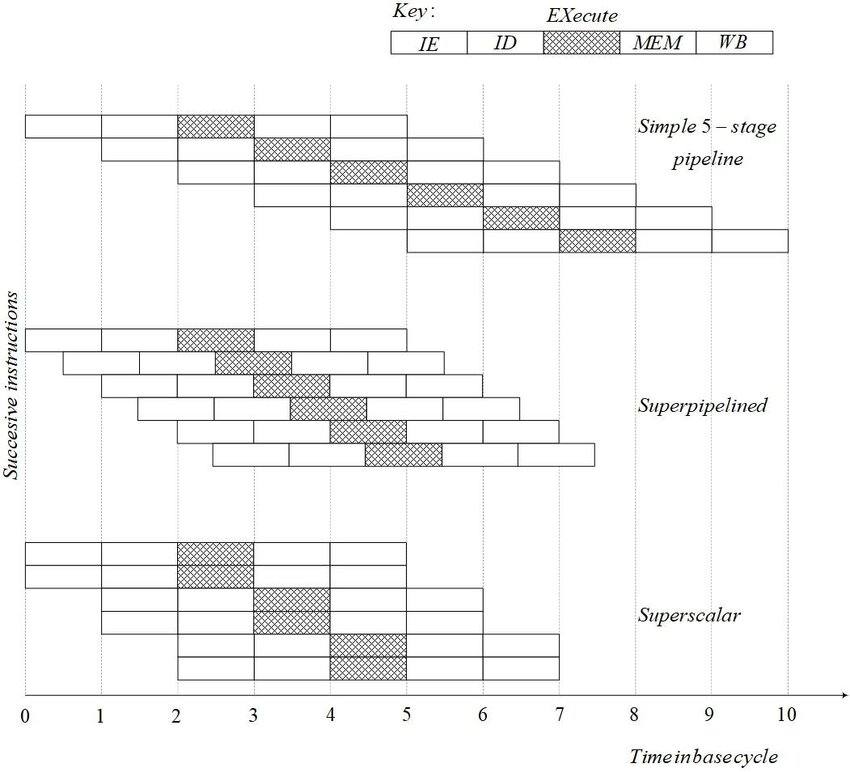
\includegraphics[width=0.5\textwidth]{SSvsSP.png}
  \caption{Superescalar contra Supersegmentado.}
\end{figure}

\subsection*{Limitaciones}

La aproximación superescalar depende de la habilidad para ejecutar múltiples instrucciones en paralelo. La expresión \textbf{paralelismo en las instrucciones} se refiere al grado en el que, en promedio, las instrucciones de un programa se pueden ejecutar en paralelo. Para maximizar el paralelismo en las instrucciones, se puede usar una combinación de optimizaciones realizadas por el compilador y de técnicas de hardware. Las principales limitaciones son:

\begin{itemize}
  \item \textbf{Dependencia de datos verdadera:} es cuando una instrucción necesita el dato producido por la primera instrucción. Si no hay dependencias, se puede captar y ejecutar dos instrucciones en paralelo. En caso de que exista esta dependencia de datos entre la primera y la segunda instrucción, se retrasa la segunda instrucción tantos ciclos de reloj como sea necesario para eliminar la dependencia.
  \item \textbf{Dependencia relativa al procedimiento:} la presencia de saltos en una secuencia de instrucciones complica el funcionamiento del cauce. Las instrucciones que siguen a una bifurcación tienen una dependencia relativa al procedimiento en ese bifurcación y no pueden ejecutarse hasta que se ejecute el salto.
  \item \textbf{Conflicto en los recursos:} Un conflicto en un recurso es una pugna de dos o más instrucciones por el mismo recurso al mismo tiempo. Desde el punto de vista del cauce segmentado, un conflicto en los recursos presenta el mismo comportamiento que una dependencia de datos. No obstante, hay algunas diferencias. Los conflictos en los recursos pueden superarse duplicando estos. Además, cuando una operación tarda mucho tiempo en finalizar, los conflictos en los recursos se pueden minimizar segmentando la unidad funcional apropiada.
  \item \textbf{Dependencia de salida.}
  \item \textbf{Antidependencia:} la restricción es similar a la de la dependencia verdadera pero a la inversa. En lugar de que la primera instrucción produzca un valor que usa la segunda instrucción, la segunda instrucción destruye un valor que utiliza la primera instrucción.
\end{itemize}

\subsection{Cuestiones relacionadas con el diseño}

\subsubsection*{Paralelismo en las instrucciones y paralelismo de la máquina}

El \textbf{paralelismo en las instrucciones} existe cuando las instrucciones de una secuencia son independientes y por tanto pueden ejecutarse en paralelo solapándose.

El paralelismo en las instrucciones depende de la frecuencia de dependencias de datos verdaderas y dependencias relativas al procedimiento que haya en el código. Estos factores dependen a su vez de la arquitectura del repertorio de instrucciones y de la aplicación.

El \textbf{paralelismo de la máquina} es una medida de la capacidad del procesador para sacar partido al paralelismo en las instrucciones. El paralelismo de maquina depende del número de instrucciones que pueden captarse y ejecutarse al mismo tiempo y de la velocidad y sofisticación de los mecanismos que usa el procesador para localizar instrucciones independientes.

\subsubsection*{Políticas de emisión de instrucciones}

Se utiliza el término \textbf{emisión de instrucciones} para referirse al proceso de iniciar la ejecución de instrucciones en las unidades funcionales del procesador y el término \textbf{política de emisión de instrucciones} para referirse al protocolo usado para emitir instrucciones.

El procesador intenta localizar instrucciones más allá del punto de ejecución en curso que puedan introducirse en el cauce y ejecutarse. Hay tres ordenaciones importantes:

\begin{itemize}
  \item El orden en que se captan las instrucciones.
  \item El orden en que se ejecutan las instrucciones.
  \item El orden en que las instrucciones actualizan los contenidos de los registros y de las posiciones de memoria.
\end{itemize}

Cuanto más sofisticado sea el procesador, menos limitado estará por la estrecha relación entre estas ordenaciones. Para optimizar la utilización de los diversos elementos del cauce, el procesador tendrá que alterar uno o más de estos órdenes con respecto al orden que se encontraría en una ejecución secuencial estricta. La única restricción que tiene el procesador es que el resultado debe ser correcto. De este modo, el procesador tiene que acomodar las diversas dependencias y conflictos discutidos antes.

Podemos agrupar las políticas de emisión de instrucciones de los procesadores superescalares en las siguientes categorías:

\begin{itemize}
  \item \textbf{Emisión en orden y finalización en orden:} es la política de emisión más sencilla. Consiste en emitir instrucciones en el orden exacto en que lo haría una ejecución secuencial y escribir los resultados en ese mismo orden. Ni siquiera los cauces escalares siguen una política tan ingenua. No obstante, es útil considerar esta política como base con la cual comparar otras aproximaciones más sofisticadas.
  \item \textbf{Emisión en orden y finalización desordenada:} la finalización desordenada se usa en los procesadores RISC escalares para mejorar la velocidad de las instrucciones que necesitan ciclos. Con finalización desordenada, puede haber cualquier número de instrucciones en la etapa de ejecución en un momento dado, hasta alcanzar el máximo grado de paralelismo e la máquina ocupando todas la unidades funcionales. La emisión de instrucciones se para cuando hay una pugna por un recurso, una dependencia de datos o una dependencia relativa al procedimiento. Surge la \textbf{dependencia de salida}.
  \item \textbf{Emisión desordenada y finalización desordenada:} para permitir la emisión desordenada, es necesario desacoplar las etapas del cauce de decodificación y ejecución. Esto se hace mediante un buffer llamado \textbf{ventana de instrucciones}. Con esta organización, cuando un procesador termina de decodificar una instrucción, la coloca en la ventada de instrucciones. Mientras el buffer no se llene, el procesador puede continuar captando y decodificando nuevas instrucciones. Cuando una unidad funcional de la etapa de ejecución queda disponible, se puede emitir una instrucción desde la ventana de instrucciones a la etapa de ejecución. La única restricción es que el programa funcione correctamente. Por esta política surge el termino \textbf{antidependencia}.
\end{itemize}

\subsubsection*{Renombramiento de registros}

Cuando varias instrucciones compiten por el uso de los mismos registros, generando restricciones en el cauce que reducen las prestaciones. Un método para hacer frente a este tipo de conflictos de almacenamiento se basa en una solución tradicional para los conflictos en los recursos: la duplicación de recursos.

Con el \textbf{renombramiento de registros}, el hardware del procesador asigna dinámicamente los registros, que están asociados con los valores que necesitan las instrucciones en diversos instantes de tiempo. Cuando se crea un nuevo valor de registro, se asigna un nuevo registro para ese valor. Las instrucciones posteriores que accedan a ese valor como operando fuente en ese registro tienen que sufrir un proceso de renombramiento: las referencias a registros de esas instrucciones han de revisarse para referenciar el registro que contiene el valor que se necesita.

\subsubsection*{Ejecución superescalar}

El proceso de captación de instrucciones, que incluye la predicción de saltos, se usa para formar un flujo dinámico de instrucciones. Se examinan las dependencias de este flujo, y el procesador puede eliminar las que sean artificiales. En esta ventana, las instrucciones ya no forman un flujo secuencial sino que están estructuradas de acuerdo a sus dependencias de datos verdaderas. El procesador lleva a cabo la etapa de ejecución de cada instrucción en un orden determinado por las dependencias de datos verdaderas y la disponibilidad de los recursos hardware. Por último, las instrucciones se vuelven a poner conceptualmente en un orden secuencial y sus resultados se almacenan.

\begin{figure}[H]
  \centering
  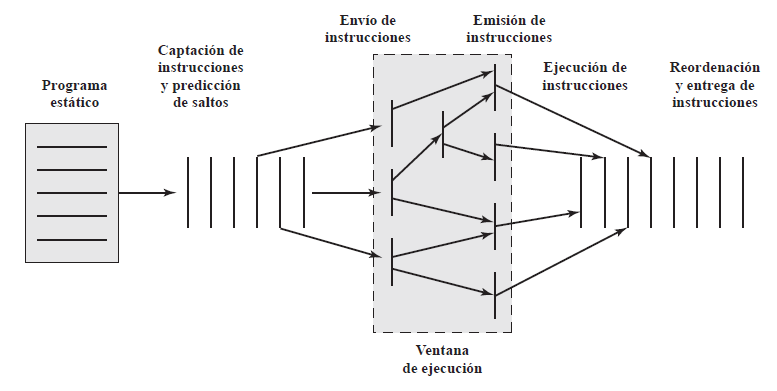
\includegraphics[width=0.7\textwidth]{ProcesamientoSE.png}
  \caption{Representación conceptual del procesamiento superescalar}
\end{figure}

\subsubsection*{Implementación superescalar}

\begin{itemize}
  \item Estrategias de captación simultánea de múltiples instrucciones.
  \item Lógica para determinar dependencias verdaderas entre valores de registros y mecanismos para comunicar esos valores.
  \item Mecanismos para iniciar o emitir múltiples instrucciones en paralelo.
  \item Recursos para la ejecución en paralelo de múltiples instrucciones.
  \item Mecanismos para entregar el estado del procesador en un orden correcto.
\end{itemize}

\subsubsection*{Consideraciones destacables en el procesamiento superescalar}

En el momento en que se produce una excepción hay varias instrucciones en ejecución. Si $I_1$ produce una excepción $\to$ ¿ha podido terminar $I_2$? $\to$ Estado inconsistente (excepciones imprecisas).

El comportamiento debería ser idéntico al que tendría la misma computadora no segmentada. Para garantizar un estado consistente:

\begin{itemize}
  \item Instrucciones anteriores terminan correctamente.
  \item La que origina la excepción y siguientes se abortan.
  \item Tras la rutina de tratamiento se comienza por la que originó la excepción.
\end{itemize}

\subsection{Pentium 4}

Aunque el concepto de diseño superescalar se asocia generalmente con la arquitectura RISC, se pueden aplicar los mismos principios superescalares a una máquina CISC.\@ El ejemplo más notable de ello tal vez sea el Pentium.

\begin{figure}[H]
  \centering
  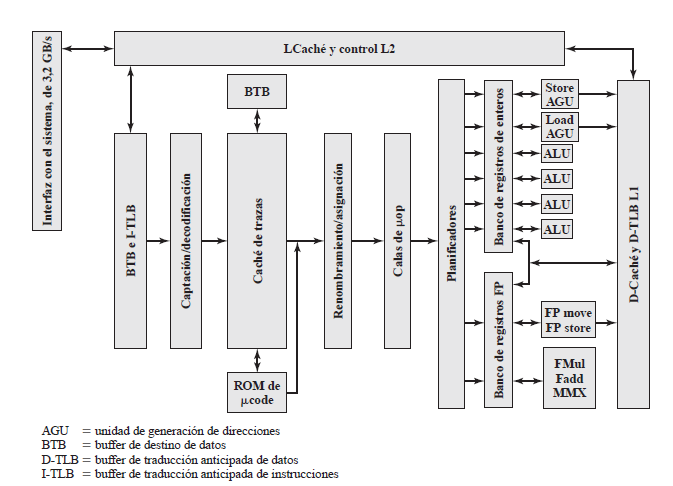
\includegraphics[width=0.6\textwidth]{Pentium4.png}
  \caption{Diagrama de bloques del Pentium 4}
\end{figure}

El funcionamiento del Pentium 4 se puede resumir como sigue:

\begin{itemize}
  \item El procesador capta instrucciones de memoria en el orden en que aparecen en el programa estático.
  \item Cada instrucción se traduce en una o más instrucciones RISC de tamaño fijo conocidas como \textbf{microoperaciones} o \textbf{micro-ops}.
  \item El procesador ejecuta las micro-ops en una organización de cauce superescalar, de modo se pueden ejecutar desordenadas.
  \item El procesador entrega los resultados de la ejecución de cada micro-op al conjunto de registros, en el orden del flujo del programa original.
\end{itemize}

En realidad, la arquitectura del Pentium 4 consta de una envoltura CISC con un núcleo RISC interno. Las micro-ops RISC internas pasan a través de un cauce con al menos veinte etapas; en algunos casos, las micro-ops necesitan múltiples etapas de ejecución, lo que se traduce en un cauce aún más largo.

\subsection{Arquitectura IA-64}

Intel se asocia con HP para desarrollar una nueva arquitectura de 64 bits, llamada IA-64. La arquitectura IA-64 no es una ampliación a 64 bits de la arquitectura de 32 bits x86 de Intel. La IA-64 aprovecha la enorme circuitería y la gran velocidad disponibles en las más recientes generaciones de microchips gracias a la utilización sistemática del paralelismo.

\subsubsection{Motivación}

Los conceptos básicos en los que se fundamenta la arquitectura IA-64 son los siguientes:

\begin{itemize}
  \item Paralelismo en las instrucciones que queda explícito en las instrucciones máquina, en lugar de depender del procesador en tiempo de ejecución.
  \item Palabras de instrucción largas o muy largas (LIW\footnote[1]{long instruction word}/VLIW\footnote[2]{very long instruction word}).
  \item Ejecución de saltos basada en predicados (concepto diferente al de predicción de saltos).
  \item Carga especulativa.
\end{itemize}

Intel y HP hacen referencia a esta combinación de conceptos con el nombre de computación con instrucciones explícitamente paralelas (EPIC). La arquitectura IA-64 consiste en un repertorio de instrucciones real destinado a ser implementado usando la tecnología EPIC.\@ El primer producto de Intel basado en IA-64 es conocido con el nombre de \textbf{Itanium}.

\begin{table}[h]
  \centering
  \begin{tblr}{
    width = \linewidth,
    colspec = {Q[462]Q[479]},
    row{1} = {c},
    hlines,
    vlines,
    }
    \textbf{Superescalar}                                                                                         & \textbf{IA-64}                                                                                                           \\
    Instrucciones de tipo RISC, una por palabra                                                                   & Instrucciones de tipo RISC puestas en grupos de tres                                                                     \\
    Multiples unidades de ejecución en paralelo                                                                   & Múltiples unidades de ejecución en paralelo                                                                              \\
    Reordena y optimiza el flujo de instrucciones en tiempo de ejecución                                          & Reordena y optimiza el flujo de instrucciones en tiempo de compilación.                                                  \\
    Predicción de saltos con ejecución especulativa de un camino.                                                 & Ejecución especulativa de los dos caminos de una bifurcación.                                                            \\
    {Carga de datos desde memoria solo cuando es necesario, e intenta encontrar los datos primero en las cachés.} & {Carga datos especulativamente antes de que se necesiten, y sigue intentando encontrar los datos primero en las cachés.}
  \end{tblr}
\end{table}

Intel y HP han propuesto un planteamiento de diseño global que permite la utilización eficaz de un procesador con muchas unidades de ejecución en paralelos. El corazón de este nuevo enfoque es el concepto de paralelismo explícito. En esta aproximación, el compilador planifica estáticamente las instrucciones en tiempo de compilación, en lugar de que lo haga dinámicamente el procesador en tiempo de ejecución. El compilador determina qué instrucciones pueden ejecutarse en paralelo e incluye esta información en la instrucción máquina. El procesador usa esa información para llevar a cabo la ejecución paralela. Una ventaja de esta aproximación es que el procesador EPIC no requiere tanta circuitería compleja como un procesador superescalar capaz de ejecutar instrucciones sin orden. Además, mientras que el procesador tiene que determinar la posibilidad de una potencial ejecución en paralelo en cuestión de nanosegundos, el compilador dispone de un plazo varios órdenes de magnitud mayor para examinar el código con detenimiento y estudiar el programa globalmente.

\subsubsection{Organización general}

Como cualquier arquitectura de procesador, la IA-64 puede implementarse con diversas organizaciones. Sus características más importantes son:

\begin{itemize}
  \item \textbf{Gran numero de registros:} el formato de instrucción de la arquitectura IA-64 supone el empleo de 256 registros, 128 registros de 64 bits de uso general para uso con enteros, con datos lógicos y para propósito general, y 128 registros de 82 bits para su uso con coma flotante y gráficos. También hay 64 bits de predicado de un bit, usados para la ejecución con predicados.
  \item \textbf{Multiples unidades de ejecución:} una máquina superescalar típica puede tener cuatro cauces paralelos, empleando cuatro unidades de ejecución en paralelo tanto para la parte de enteros del procesador como para la parte de la coma flotantes. Se espera que la IA-64 se implemente en sistemas con ocho o más unidades paralelas.
\end{itemize}

En la arquitectura IA-64 se definen cuatro tipos de unidades de ejecución:

\begin{itemize}
  \item \textbf{I:} para instrucciones aritméticas con enteros, de desplazamiento y suma, lógicas de comparación y multimedia con enteros.
  \item \textbf{M:} cargas y almacenamientos entre registros y memoria más algunas operaciones de la ALU con enteros.
  \item \textbf{B:} instrucciones de salto.
  \item \textbf{F:} instrucciones de coma flotante.
\end{itemize}

\subsubsection*{Formato de instrucción}

La arquitectura IA-64 define un \textbf{paquete} de 128 bits que contiene tres instrucciones, llamadas \textbf{silabas}, y un campo plantilla. El procesador puede captar uno o más paquetes de instrucciones a la vez; y cada captación indica qué instrucciones se pueden ejecutar en paralelo. La interpretación de este campo no se limita a un único paquete. Por el contrario, el procesador puede examinar varios paquetes para determinar qué instrucciones pueden ejecutarse en paralelo.

Las instrucciones agrupadas no tienen que estar en el orden original del programa. Además, debido a la flexibilidad del campo plantilla, el compilador puede mezclar instrucciones dependientes e independientes en el mismo paquete.

\begin{figure}[h]
  \centering
  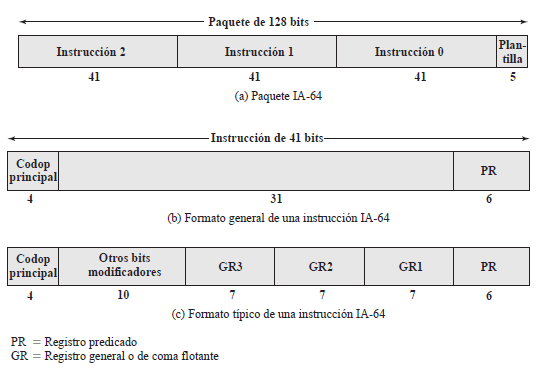
\includegraphics[width=0.6\textwidth]{InstruccionesIA-64.png}
  \caption{Formato de instrucción de la arquitectura IA-64}
\end{figure}

El valor de plantilla tiene dos propósitos:

\begin{itemize}
  \item El campo especifica la correspondencia de las instrucciones con los tipos de unidades de ejecución. No son posibles todas las correspondencias de instrucciones con unidades.
  \item El campó indica la presencia de posibles \textbf{paradas}. Una parada indica al hardware que una o más instrucciones anteriores a la parada pueden tener ciertos tipos de dependencias de recursos con una o más instrucciones posteriores a la parada.
\end{itemize}

\subsubsection*{Saltos predicados}

Los saltos predicados son una técnica de compilación. El compilador elimina saltos del programa usando ejecución condicional, es necesario soporte de hardware. Se deja que ambas ramas de un salto condicional se ejecuten en paralelo.

Procedimiento para saltos predicados:

\begin{enumerate}
  \item El procesador encuentra una instrucción de salto predicado y determina la dirección de destino de las dos posibles ramas del salto (la rama verdadera y la rama falsa).
  \item Mientras se resuelve la condición del salto, el procesador especulativamente cumple las instrucciones de ambas ramas en paralelo, manteniendo un estado interno de ejecución especulativa.
  \item Se realiza la evaluación de la condición del salto. Si la condición se determina como verdadera, el procesador descarta los resultados de la rama falsa y continúa la ejecución en la rama verdadera. Si la condición es falsa, se descartan los resultados de la rama verdadera y se continúa en la rama falsa.
  \item Los resultados correctos de la rama seleccionada se reescriben en los registros y se continúa la ejecución secuencial a partir de la instrucción de destino correspondiente.
\end{enumerate}